\chapter{Spectroscopy for Structure}\label{ch:b1:structure-spectroscopy}

A perfumer hands the laboratory a colourless liquid that smells of
pineapple and asks what it is. Fifty years ago, the answer would have
taken weeks of degradation reactions. Today it takes ten minutes: an
elemental analysis gives the formula, an infrared spectrum names the
functional group, and a proton nuclear magnetic resonance spectrum shows
how the atoms are joined. This chapter explains how each spectrum is
read --- what light of each region does to a molecule, and which
features of a spectrum carry which piece of structure --- and ends with
that pineapple molecule.

\begin{recall}
The school volume (grades 11 and 12) measured \omterm{def:b1:structure-spectroscopy:absorbance}{absorbances} with a
spectrophotometer and used the Beer--Lambert law to find concentrations,
identified functional groups from tables of infrared bands, and read
simple proton NMR spectra (number of signals, \omterm{def:b1:structure-spectroscopy:integration}{integration}, the $n + 1$
rule). Single, double and triple bonds and the $\pi$ bond are those of
\cref{ch:b1:lewis-resonance-vsepr}.
\end{recall}

\section{UV--visible spectroscopy: conjugation and colour}

\begin{definition}[Absorbance and the Beer--Lambert law]\label{def:b1:structure-spectroscopy:absorbance}
For light of intensity $I_0$ entering a solution and $I$ leaving it, the
\emph{absorbance}\index{absorbance} is $A = \log(I_0/I)$. For a dilute
solution of one absorbing species, $A = \varepsilon\,\ell\,c$ (the
Beer--Lambert law), where $\ell$ is the path length, $c$ the
concentration and $\varepsilon$ the \emph{molar absorption
coefficient}\index{molar absorption coefficient}, a property of the
species at that wavelength.
\end{definition}

A molecule absorbs ultraviolet or visible light when a photon's energy
matches the gap between the highest occupied and the lowest empty
electron levels of its bonds. For $\sigma$ bonds the gap is large and the
absorption lies far in the ultraviolet; $\pi$ bonds absorb closer to the
visible, and a chain of alternating double and single bonds absorbs at
longer wavelengths the longer the chain.

\begin{definition}[Conjugated system, chromophore, absorption maximum]\label{def:b1:structure-spectroscopy:conjugation}
A \emph{conjugated system}\index{conjugated system} is a chain of atoms
each carrying a $p$ orbital in a $\pi$ system, as in alternating
double and single bonds (buta-1,3-diene, benzene). The group of atoms
responsible for an absorption is its \emph{chromophore}\index{chromophore};
the wavelength at which its \omterm{def:b1:structure-spectroscopy:absorbance}{absorbance} is greatest is the
\emph{absorption maximum}\index{absorption maximum}, $\lambda_{\max}$.
\end{definition}

The levels of a \omterm{def:b1:structure-spectroscopy:conjugation}{conjugated system} spread over the whole chain and come
closer together as the chain grows, as the levels of a particle in a
longer box do: $\lambda_{\max}$ increases with conjugation. Ethene and
butadiene absorb in the ultraviolet only; the eleven conjugated double
bonds of $\beta$-carotene bring the absorption into the blue part of the
visible. A substance looks the colour complementary to the light it
absorbs: absorbing blue and violet, carotene looks orange.

\begin{omfigure}
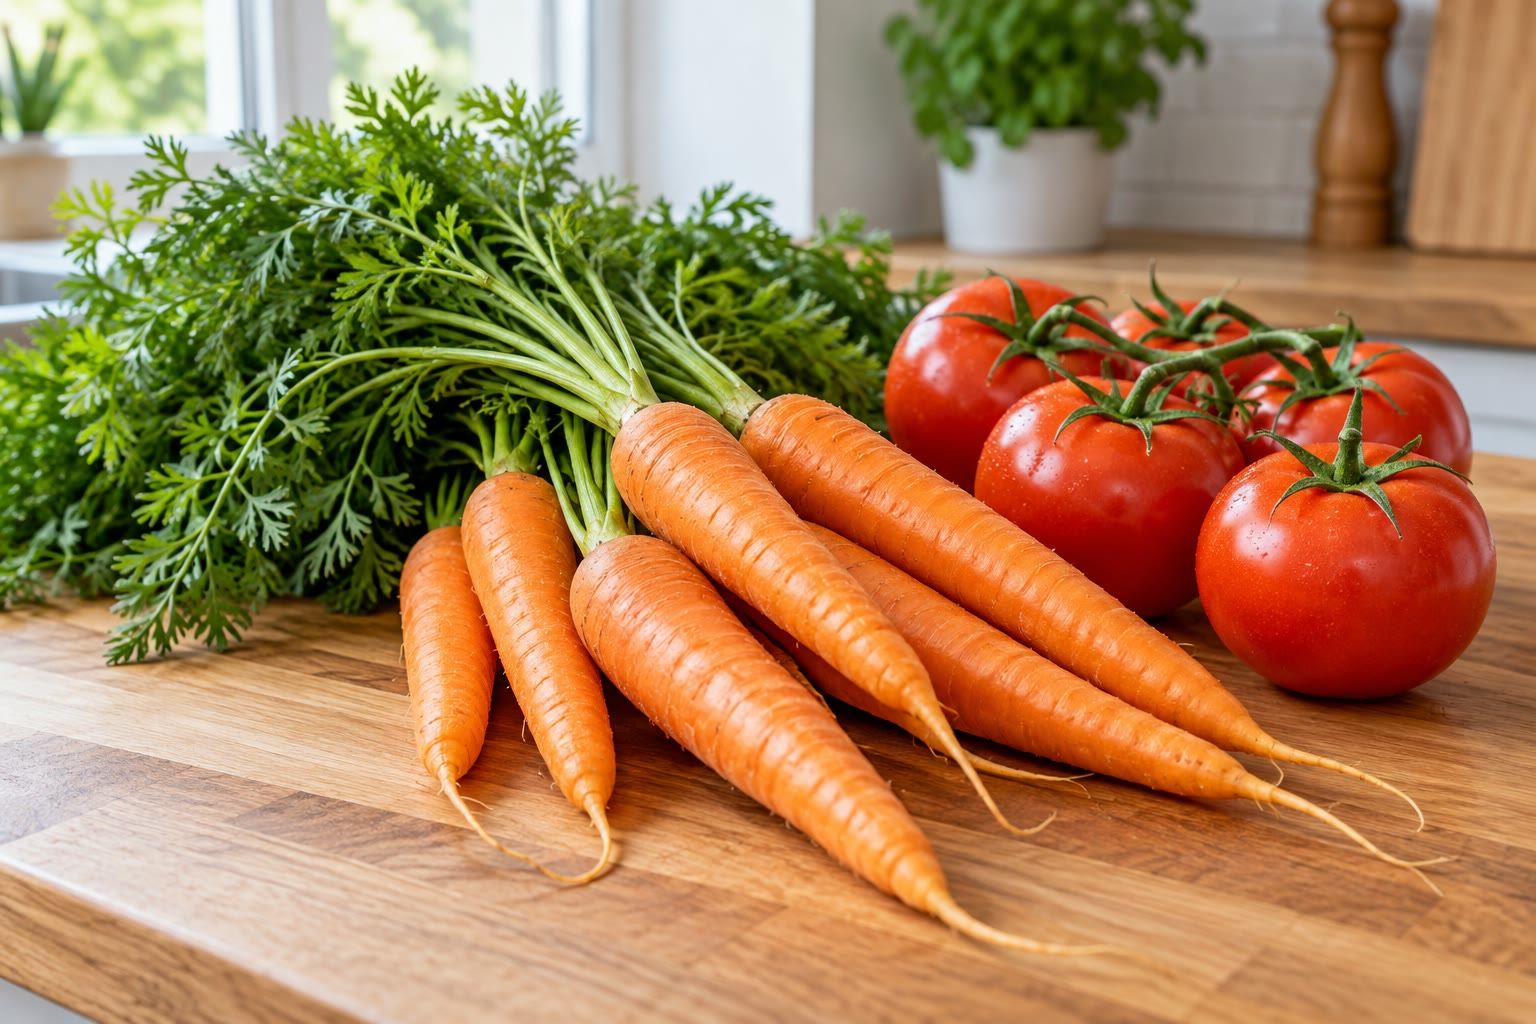
\includegraphics[width=0.55\linewidth]{images/book2/ai/b1-17-carrots-tomatoes.jpg}

{\small Carrots and tomatoes owe their colours to long conjugated
molecules, carotenes and lycopene, that absorb blue and green light and
let orange and red through.}
\end{omfigure}

\begin{omfigure}
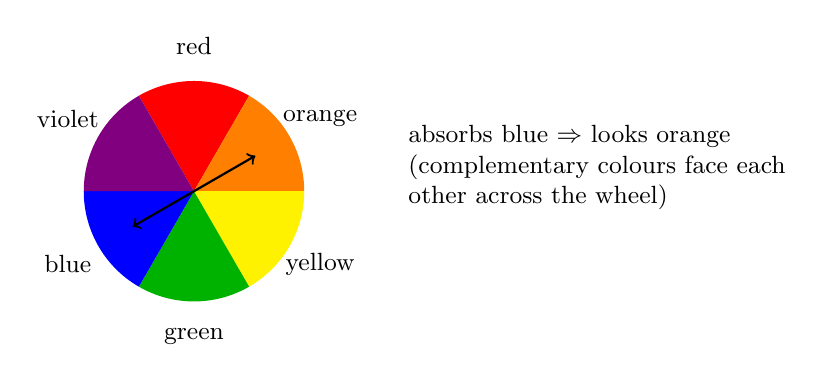
\begin{tikzpicture}[font=\small]
  \foreach \a/\c/\n in {90/red/red, 30/orange/orange, -30/yellow/yellow, -90/green!70!black/green, -150/blue/blue, 150/violet/violet} {
    \fill[\c] (0,0) -- (\a-30:1.4) arc[start angle=\a-30, end angle=\a+30, radius=1.4] -- cycle;
    \node at (\a:1.85) {\n};
  }
  \draw[<->, thick] (-150:0.9) -- (30:0.9);
  \node[align=left, anchor=west] at (2.6,0.3) {absorbs blue $\Rightarrow$ looks orange\\(complementary colours face each\\other across the wheel)};
\end{tikzpicture}

{\small A colour wheel. The colour seen is the complement of the colour
absorbed: a solution absorbing in the blue looks orange.}
\end{omfigure}

\section{Infrared spectroscopy in depth}

\begin{definition}[Wavenumber, transmittance, fingerprint region]\label{def:b1:structure-spectroscopy:wavenumber}
Infrared spectra are plotted against the \emph{wavenumber}\index{wavenumber}
$\tilde\nu = 1/\lambda$, in \unit{cm^{-1}}, proportional to the energy of the
photon. The ordinate is the \emph{transmittance}\index{transmittance}
$T = I/I_0$, in per cent, so that bands point downwards. Below about
\qty{1500}{cm^{-1}} many overlapping bands, characteristic of the whole
molecule rather than of one bond, form the \emph{fingerprint
region}\index{fingerprint region}.
\end{definition}

A bond absorbs infrared light at the frequency at which it vibrates. As
for two masses joined by a spring, the stiffer the bond and the lighter
the atoms, the higher the \omterm{def:b1:structure-spectroscopy:wavenumber}{wavenumber}: bonds to hydrogen (O--H, C--H)
above \qty{2800}{cm^{-1}}, triple bonds near 2200, double bonds near
1700--1600, single bonds between heavier atoms below 1300. The table gives
measured positions for the molecules of this chapter, in the gas \omterm{def:b1:extent-q-and-k:system}{phase},
where the molecules are isolated.

\begin{omfigure}
\begin{tabular}{llr}
\hline
molecule & bond & $\tilde\nu$ (\unit{cm^{-1}}) \\
\hline
ethanol & O--H & 3666 \\
ethanol & C--H & 2978 \\
ethanol & C--O & 1060 \\
propanone & C=O & 1738 \\
ethanoic acid & O--H & 3582 \\
ethanoic acid & C=O & 1788 \\
ethyl ethanoate & C=O & 1764 \\
ethyl ethanoate & C--O & 1238 \\
\hline
\end{tabular}

\smallskip
{\small Band maxima in \omterm{def:b1:extent-q-and-k:system}{gas-phase} infrared spectra. In liquids, \omterm{def:b1:intermolecular-forces-solvents:hbond}{hydrogen
bonds} broaden the O--H bands and move them to lower \omterm{def:b1:structure-spectroscopy:wavenumber}{wavenumbers}, and the
C=O bands of acids move down as the acid pairs up.}
% ledger: ir:ethanol-OH, ir:ethanol-CH, ir:ethanol-CO, ir:propanone-CO, ir:ethanoic-OH, ir:ethanoic-CO, ir:ethylethanoate-CO, ir:ethylethanoate-COC
\end{omfigure}

\begin{omfigure}
\begin{tikzpicture}
\begin{axis}[name=i1, width=0.86\linewidth, height=3.2cm, xmin=500, xmax=4000, x dir=reverse, ymin=0, ymax=105, ytick={0,50,100}, ylabel={$T$ (\%)}, tick label style={font=\scriptsize}, label style={font=\small}, xticklabels={}]
\addplot[omDef, thick] table[x=nu, y=T] {figdata/out/bachelor-1-spectra-ir-ethanol.dat};
\node[font=\scriptsize, anchor=west] at (axis cs:2600,25) {ethanol};
\end{axis}
\begin{axis}[name=i2, at={(i1.south)}, anchor=north, yshift=-0.25cm, width=0.86\linewidth, height=3.2cm, xmin=500, xmax=4000, x dir=reverse, ymin=0, ymax=105, ytick={0,50,100}, ylabel={$T$ (\%)}, tick label style={font=\scriptsize}, label style={font=\small}, xticklabels={}]
\addplot[omProp, thick] table[x=nu, y=T] {figdata/out/bachelor-1-spectra-ir-propanone.dat};
\node[font=\scriptsize, anchor=west] at (axis cs:2600,25) {propanone};
\end{axis}
\begin{axis}[at={(i2.south)}, anchor=north, yshift=-0.25cm, width=0.86\linewidth, height=3.2cm, xmin=500, xmax=4000, x dir=reverse, ymin=0, ymax=105, ytick={0,50,100}, ylabel={$T$ (\%)}, tick label style={font=\scriptsize}, label style={font=\small}, xlabel={wavenumber (\unit{cm^{-1}})}]
\addplot[omMeth, thick] table[x=nu, y=T] {figdata/out/bachelor-1-spectra-ir-ethanoic.dat};
\node[font=\scriptsize, anchor=west] at (axis cs:2600,25) {ethanoic acid};
\end{axis}
\end{tikzpicture}

{\small Infrared spectra of ethanol, propanone and ethanoic acid,
simulated from the measured band positions of the table (band heights and
widths schematic). The C=O band near \qty{1750}{cm^{-1}} and the O--H band
above \qty{3500}{cm^{-1}} tell the three functional groups apart at a
glance.}
\end{omfigure}

\section{Proton NMR: chemical shift and integration}

In a strong magnetic field, a proton has two \omterm{def:b1:quantum-numbers:energy-level}{energy levels}; radio waves
of the right frequency make it flip from one to the other. That frequency
is proportional to the magnetic field the proton actually feels, which
the electrons around it reduce slightly. Protons in different chemical
environments therefore resonate at slightly different frequencies.

\begin{definition}[Chemical shift, shielding, equivalent protons]\label{def:b1:structure-spectroscopy:chemical-shift}
The \emph{chemical shift}\index{chemical shift} of a proton is
$\delta = (\nu - \nu_{\text{ref}})/\nu_0 \times 10^6$, in \unit{ppm}, where
$\nu$ is its resonance frequency, $\nu_{\text{ref}}$ that of the protons
of tetramethylsilane and $\nu_0$ the operating frequency of the
spectrometer. The reduction of the field at a nucleus by its electrons is
its \emph{shielding}\index{shielding}: electron-withdrawing neighbours
(O, halogens, C=O) deshield a proton and raise its $\delta$.
\emph{Equivalent protons}\index{equivalent protons} are protons exchanged
by a symmetry of the molecule or by a fast rotation; they have the same
shift.
\end{definition}

\begin{proposition}[The shift does not depend on the spectrometer]\label{prop:b1:structure-spectroscopy:shift-field-independent}
The \omterm{def:b1:structure-spectroscopy:chemical-shift}{chemical shift} of a proton is the same on spectrometers of different
fields.
\end{proposition}

\begin{proof}
Both $\nu$ and $\nu_{\text{ref}}$ are proportional to the applied field
$B_0$ (each multiplied by its own \omterm{def:b1:structure-spectroscopy:chemical-shift}{shielding} factor), and so is $\nu_0$.
The ratio $(\nu - \nu_{\text{ref}})/\nu_0$ is therefore independent of
$B_0$. Differences in hertz, by contrast, grow with the field.
\end{proof}

\begin{definition}[Integration]\label{def:b1:structure-spectroscopy:integration}
The \emph{integration}\index{integration} of a signal is its area, read
on the spectrum as the height of a step curve; areas are proportional to
the numbers of protons giving the signals.
\end{definition}

\section{Spin--spin coupling}

\begin{definition}[Spin--spin coupling, coupling constant, multiplet]\label{def:b1:structure-spectroscopy:coupling}
Through the bonds, the magnetic state of a proton slightly changes the
field felt by protons on the neighbouring carbons: this
\emph{spin--spin coupling}\index{spin--spin coupling} splits each signal
into a \emph{multiplet}\index{multiplet} of lines separated by the
\emph{coupling constant}\index{coupling constant} $J$, in hertz. Two
protons coupled to each other show the same $J$; \omterm{def:b1:structure-spectroscopy:chemical-shift}{equivalent protons} do
not split each other's signal.
\end{definition}

\begin{proposition}[The \texorpdfstring{$n + 1$}{n + 1} rule]\label{prop:b1:structure-spectroscopy:n-plus-one}
A proton (or a set of \omterm{def:b1:structure-spectroscopy:chemical-shift}{equivalent protons}) coupled with the same $J$ to
$n$ equivalent neighbours gives $n + 1$ lines, separated by $J$, of
relative intensities the binomial coefficients $\binom{n}{k}$, $k = 0$ to
$n$ (the \emph{$n + 1$ rule}\index{$n + 1$ rule}).
\end{proposition}

\begin{proof}
Each neighbour is in one of two spin states, shifting the observed line by
$+J/2$ or $-J/2$. With $n$ neighbours the shift is $(k - n/2)J$, where $k$
is the number in the first state: $n + 1$ values, equally spaced by $J$.
The two states being almost equally populated, all $2^n$ combinations
are equally likely, and $k$ of them in the first state happens in
$\binom{n}{k}$ ways.
\end{proof}

\begin{omfigure}
\begin{tikzpicture}[font=\small, x=0.85cm, y=0.5cm]
  % quartet: three neighbours, each split +-J/2 (J = 1.5 units)
  \draw[thick] (0,4) -- (0,3.4);
  \foreach \x in {-0.75,0.75} \draw (0,3.4) -- (\x,2.4);
  \foreach \a/\b in {-0.75/-1.5, -0.75/0, 0.75/0, 0.75/1.5} \draw (\a,2.4) -- (\b,1.4);
  \foreach \a/\b in {-1.5/-2.25, -1.5/-0.75, 0/-0.75, 0/0.75, 1.5/0.75, 1.5/2.25} \draw (\a,1.4) -- (\b,0.4);
  \foreach \x/\h in {-2.25/1, -0.75/3, 0.75/3, 2.25/1} {\draw[omDef, very thick] (\x,-2.6) -- (\x,{-2.6+0.7*\h}); \draw[dotted] (\x,0.4) -- (\x,{-2.6+0.7*\h});}
  \draw (-2.8,-2.6) -- (2.8,-2.6);
  \node at (0,-3.4) {quartet 1\,:\,3\,:\,3\,:\,1 (\ce{-CH2-} next to \ce{-CH3})};
  % triplet: two neighbours
  \begin{scope}[xshift=7.5cm]
  \draw[thick] (0,4) -- (0,3.4);
  \foreach \x in {-0.75,0.75} \draw (0,3.4) -- (\x,2.4);
  \foreach \a/\b in {-0.75/-1.5, -0.75/0, 0.75/0, 0.75/1.5} \draw (\a,2.4) -- (\b,1.4);
  \foreach \x/\h in {-1.5/1, 0/2, 1.5/1} {\draw[omProp, very thick] (\x,-2.6) -- (\x,{-2.6+0.7*\h}); \draw[dotted] (\x,1.4) -- (\x,{-2.6+0.7*\h});}
  \draw (-2.1,-2.6) -- (2.1,-2.6);
  \draw[<->] (-1.5,-0.6) -- (0,-0.6) node[midway, above, font=\scriptsize] {$J$};
  \node at (0,-3.4) {triplet 1\,:\,2\,:\,1 (\ce{-CH3} next to \ce{-CH2-})};
  \end{scope}
\end{tikzpicture}

{\small Splitting trees. Each neighbour splits every line into two, $J$
apart; coinciding lines add up, giving the binomial intensities.}
\end{omfigure}

\begin{omfigure}
\begin{tikzpicture}
\begin{axis}[name=ea,
  width=0.86\linewidth, height=4.2cm, xmin=0.8, xmax=4.5, x dir=reverse, ymin=0, ymax=1.15,
  axis x line=bottom, axis y line=none, xlabel={$\delta$ (ppm)},
  tick label style={font=\scriptsize}, label style={font=\small}]
\addplot[omDef, thin] table[x=ppm, y=I] {figdata/out/bachelor-1-spectra-nmr-ethylethanoate.dat};
\node[font=\scriptsize, anchor=south] at (axis cs:4.12,0.75) {q, 2H};
\node[font=\scriptsize, anchor=west] at (axis cs:2.0,0.95) {s, 3H};
\node[font=\scriptsize, anchor=west] at (axis cs:1.15,0.8) {t, 3H};
\node[font=\small, anchor=north east] at (axis cs:3.4,1.1) {\ce{CH3COOCH2CH3}};
\end{axis}
\begin{axis}[at={(ea.south)}, anchor=north, yshift=-1.3cm,
  width=0.86\linewidth, height=4.2cm, xmin=0.8, xmax=4.5, x dir=reverse, ymin=0, ymax=1.15,
  axis x line=bottom, axis y line=none, xlabel={$\delta$ (ppm)},
  tick label style={font=\scriptsize}, label style={font=\small}]
\addplot[omProp, thin] table[x=ppm, y=I] {figdata/out/bachelor-1-spectra-nmr-ethanol.dat};
\node[font=\scriptsize, anchor=south] at (axis cs:3.69,0.75) {q, 2H};
\node[font=\scriptsize, anchor=west] at (axis cs:2.55,0.6) {s, 1H};
\node[font=\scriptsize, anchor=west] at (axis cs:1.1,0.8) {t, 3H};
\node[font=\small, anchor=north east] at (axis cs:3.2,1.1) {\ce{CH3CH2OH}};
\end{axis}
\end{tikzpicture}

{\small Proton NMR spectra of ethyl ethanoate (top) and ethanol (bottom)
in \ce{CDCl3}, simulated at \qty{90}{MHz} from measured shifts and
\omterm{def:b1:structure-spectroscopy:coupling}{coupling constants} ($J = \qty{7.2}{Hz}$ and \qty{7.0}{Hz}). The
\ce{OCH2} quartet is deshielded by the oxygen; in ethanol the OH proton,
exchanged quickly between molecules, does not couple and its shift
depends on the concentration.}
% ledger: nmr:ethylethanoate-OCH2, nmr:ethylethanoate-COCH3, nmr:ethylethanoate-CH3, nmr:ethylethanoate-J, nmr:ethanol-CH2, nmr:ethanol-CH3, nmr:ethanol-OH, nmr:ethanol-J
\end{omfigure}

\begin{omfigure}
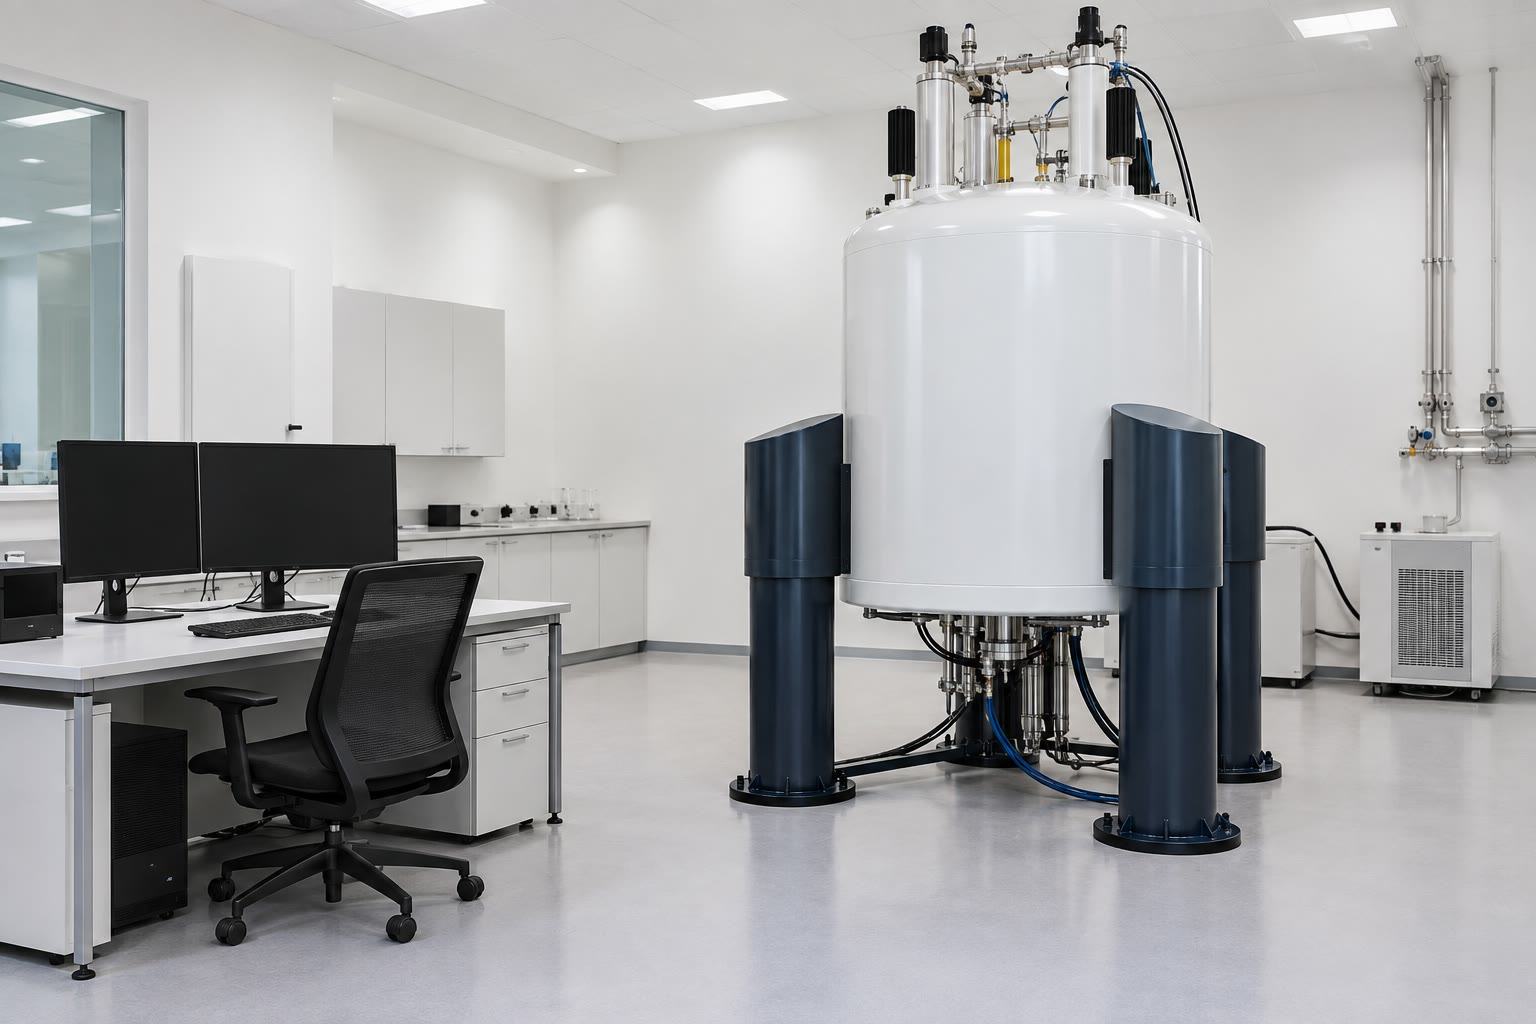
\includegraphics[width=0.5\linewidth]{images/book2/ai/b1-17-nmr.jpg}

{\small An NMR spectrometer: the tall cylinder holds a superconducting
magnet cooled by liquid helium; the sample tube is lowered into its
centre.}
\end{omfigure}

\section{Solving a structure}

\begin{definition}[Degree of unsaturation]\label{def:b1:structure-spectroscopy:unsaturation}
The \emph{degree of unsaturation}\index{degree of unsaturation} of a
formula is the number of rings plus the number of $\pi$ bonds in the
molecule.
\end{definition}

\begin{proposition}[Degree of unsaturation from the formula]\label{prop:b1:structure-spectroscopy:unsaturation-formula}
For a molecule $\mathrm{C}_c\mathrm{H}_h\mathrm{N}_n\mathrm{O}_o\mathrm{X}_x$
(X a halogen), the \omterm{def:b1:structure-spectroscopy:unsaturation}{degree of unsaturation} is
\[
  D = \frac{2c + 2 + n - h - x}{2} .
\]
\end{proposition}

\begin{proof}
An open chain of $c$ carbons with only single bonds carries $2c + 2$
hydrogens. Each ring or $\pi$ bond removes two of them. A divalent oxygen
inserted in a chain changes nothing; a trivalent nitrogen brings one more
hydrogen; a halogen takes the place of one hydrogen. Counting the
hydrogens missing and dividing by two gives $D$.
\end{proof}

\begin{method}[Solving a structure]\label{met:b1:structure-spectroscopy:solve-structure}
\begin{enumerate}
  \item From the formula, compute $D$.
  \item From the IR spectrum, find the functional groups (C=O, O--H, N--H,
        C--O) and the absence of others.
  \item From the NMR spectrum: number of signals (sets of \omterm{def:b1:structure-spectroscopy:chemical-shift}{equivalent
        protons}), \omterm{def:b1:structure-spectroscopy:integration}{integrations} (protons per set), shifts (neighbouring
        groups), multiplicities (number of neighbours by the $n + 1$
        rule), \omterm{def:b1:structure-spectroscopy:coupling}{coupling constants} (which signals are neighbours).
  \item Build fragments, join them, and check every peak against the
        proposed structure; discard the isomers that disagree.
\end{enumerate}
\end{method}

\section{Exercises}

\begin{exercise}[$\star$]\label{exo:b1:structure-spectroscopy:1}
A solution of a dye at \qty{2.0e-5}{mol/L} in a \qty{1.00}{cm} cell has
an \omterm{def:b1:structure-spectroscopy:absorbance}{absorbance} of 0.64 at its \omterm{def:b1:structure-spectroscopy:conjugation}{absorption maximum}. Compute $\varepsilon$, and
the \omterm{def:b1:structure-spectroscopy:absorbance}{absorbance} of a solution three times more concentrated.
\end{exercise}

\begin{exercise}[$\star$]\label{exo:b1:structure-spectroscopy:2}
Compute the \omterm{def:b1:structure-spectroscopy:unsaturation}{degree of unsaturation} of \ce{C6H6}, \ce{C4H8O2}, \ce{C3H7NO},
\ce{C2H3Cl} and \ce{C10H14O} (carvone). Propose one structure for each.
\end{exercise}

\begin{exercise}[$\star$]\label{exo:b1:structure-spectroscopy:3}
How many proton signals, with which \omterm{def:b1:structure-spectroscopy:integration}{integrations}, do propanone, ethanoic
acid, 2-methylpropane and 1,2-dichloroethane give?
\end{exercise}

\begin{exercise}[$\star$]\label{exo:b1:structure-spectroscopy:4}
A signal lies \qty{1460}{Hz} from tetramethylsilane on a
\qty{400}{MHz} spectrometer. What is its shift? How far in hertz would it
be at \qty{90}{MHz}? Why do high fields separate \omterm{def:b1:structure-spectroscopy:coupling}{multiplets} better?
\end{exercise}

\begin{exercise}[$\star\star$]\label{exo:b1:structure-spectroscopy:5}
Predict the multiplicity of each signal of 1-bromopropane,
\ce{CH3CH2CH2Br}, assuming equal \omterm{def:b1:structure-spectroscopy:coupling}{coupling constants}, and the relative
intensities of the lines of the central signal.
\end{exercise}

\begin{exercise}[$\star\star$]\label{exo:b1:structure-spectroscopy:6}
How do the IR spectra of ethanol, propanone and ethanoic acid differ
between 1700 and \qty{3700}{cm^{-1}}? Which one compound gives both
a C=O and an O--H band?
\end{exercise}

\begin{exercise}[$\star\star$]\label{exo:b1:structure-spectroscopy:7}
Two isomers \ce{C4H8O2}: ethyl ethanoate and methyl propanoate. Predict
their NMR spectra (shifts approximately, multiplicities, \omterm{def:b1:structure-spectroscopy:integration}{integrations})
and say how to tell them apart.
\end{exercise}

\begin{exercise}[$\star\star$]\label{exo:b1:structure-spectroscopy:8}
Using the simulated spectrum of ethyl ethanoate, read the separation of
two lines of the quartet in ppm and convert it to hertz (the spectrum is
simulated at \qty{90}{MHz}). Compare with the triplet.
\end{exercise}

\begin{exercise}[$\star\star$]\label{exo:b1:structure-spectroscopy:9}
A compound \ce{C3H6O} shows a strong IR band at \qty{1738}{cm^{-1}} and a
single NMR signal. Identify it. Which isomer would show a band near
\qty{2720}{cm^{-1}} and a signal near \qty{9.8}{ppm}?
\end{exercise}

\begin{exercise}[$\star\star\star$]\label{exo:b1:structure-spectroscopy:10}
Prove the $n + 1$ rule in the form: a proton coupled to two different
sets of neighbours, $n_1$ with $J_1$ and $n_2$ with $J_2$, gives $(n_1 +
1)(n_2 + 1)$ lines. When $J_1 = J_2$, how many distinct lines are left?
Apply to the central \ce{CH2} of 1-bromopropane.
\end{exercise}

\begin{exercise}[$\star\star\star$]\label{exo:b1:structure-spectroscopy:11}
A compound \ce{C4H10O} gives no IR band at 1700--1800 but a broad band
near \qty{3350}{cm^{-1}} in the liquid, and an NMR spectrum with a doublet
(6H), a \omterm{def:b1:structure-spectroscopy:coupling}{multiplet} (1H), a doublet (2H) and a broad singlet (1H). Find
the structure.
\end{exercise}

\begin{exercise}[$\star\star\star$]\label{exo:b1:structure-spectroscopy:12}
Show that the \omterm{def:b1:structure-spectroscopy:absorbance}{absorbance} of a mixture of two species obeys $A = \ell(\varepsilon_1c_1
+ \varepsilon_2c_2)$, and explain how measurements at two wavelengths give
both concentrations.
\end{exercise}

\section{Problem: The Pineapple Molecule}

\begin{problem}[{Weekend problem --- combustion analysis and vapour
density, the infrared spectrum, the proton NMR spectrum, and the
structure and molar mass of the pineapple-smelling ester}]
\label{pb:b1:structure-spectroscopy:1}
The unknown is a liquid containing only C, H and O. The combustion of
\qty{0.2500}{g} gives \qty{0.5690}{g} of carbon dioxide and
\qty{0.2328}{g} of water. Its vapour has a density of \qty{3.74}{g/L} at
\qty{100}{\celsius} and \qty{1.000}{bar}. \omterm{def:b1:extent-q-and-k:system}{Gas-phase} IR bands: 2982,
1754, \qty{1182}{cm^{-1}} (strong), none above
\qty{3100}{cm^{-1}}. Proton NMR (\ce{CDCl3}): 4.13 (q, 2H, $J = \qty{7.2}{Hz}$),
2.28 (t, 2H), 1.66 (sextet, 2H), 1.25 (t, 3H, $J = \qty{7.2}{Hz}$), 0.95
(t, 3H) ppm. $M$: C 12.0, H 1.0, O \qty{16.0}{g/mol}; $R =
\qty{8.314}{J/(K.mol)}$.
% ledger: ir:ethylbutanoate-CH, ir:ethylbutanoate-CO, ir:ethylbutanoate-COC, nmr:ethylbutanoate-OCH2, nmr:ethylbutanoate-CH2CO, nmr:ethylbutanoate-CH2, nmr:ethylbutanoate-OCH2CH3, nmr:ethylbutanoate-CH3, nmr:ethylbutanoate-J

\begin{center}
\begin{tikzpicture}
\begin{axis}[width=0.86\linewidth, height=4.0cm, xmin=0.6, xmax=4.5, x dir=reverse, ymin=0, ymax=1.15,
  axis x line=bottom, axis y line=none, xlabel={$\delta$ (ppm)},
  tick label style={font=\scriptsize}, label style={font=\small}]
\addplot[omDef, thin] table[x=ppm, y=I] {figdata/out/bachelor-1-spectra-nmr-ethylbutanoate.dat};
\end{axis}
\end{tikzpicture}
\end{center}

\medskip
\noindent\textbf{Part I --- The formula.}
\begin{enumerate}
  \item Compute the mass of carbon in the sample.
  \item Compute the mass of hydrogen.
  \item Deduce the mass of oxygen.
  \item Compute the mass percentages of C, H and O.
  \item Find the empirical formula.
  \item From the vapour density, compute the molar mass (ideal gas).
  \item Give the molecular formula and its \omterm{def:b1:structure-spectroscopy:unsaturation}{degree of unsaturation}.
\end{enumerate}

\medskip
\noindent\textbf{Part II --- The infrared spectrum.}
\begin{enumerate}[resume]
  \item Assign the band at \qty{1754}{cm^{-1}}.
  \item What does the absence of bands above \qty{3100}{cm^{-1}} exclude?
  \item Assign the strong band at \qty{1182}{cm^{-1}}.
  \item Assign the band at \qty{2982}{cm^{-1}}.
  \item With the \omterm{def:b1:structure-spectroscopy:unsaturation}{degree of unsaturation}, which family of compounds
        remains? Why not a carboxylic acid, a ketone with an ether, or a
        cyclic diol?
\end{enumerate}

\medskip
\noindent\textbf{Part III --- The NMR spectrum.}
\begin{enumerate}[resume]
  \item How many sets of \omterm{def:b1:structure-spectroscopy:chemical-shift}{equivalent protons}? Check the total \omterm{def:b1:structure-spectroscopy:integration}{integration}.
  \item Interpret the quartet at 4.13 ppm: neighbours and environment.
  \item Interpret the triplet at 1.25 ppm. Why do the two share the same
        $J$?
  \item Interpret the triplet at 2.28 ppm.
  \item Interpret the sextet at 1.66 ppm.
  \item Interpret the triplet at 0.95 ppm.
  \item Build the two fragments that these signals describe.
  \item Why are the signals at 4.13 and 2.28 ppm the most deshielded?
\end{enumerate}

\medskip
\noindent\textbf{Part IV --- The structure.}
\begin{enumerate}[resume]
  \item Join the fragments through the ester group: two possibilities.
        Which is consistent with the shifts?
  \item Explain why propyl propanoate does not fit.
  \item Explain why butyl ethanoate does not fit.
  \item Name the compound and draw its structure.
  \item Check each IR band and each NMR signal against the structure.
  \item State the molar mass of the pineapple molecule.
\end{enumerate}
\end{problem}
